%%%%%%%%%%%%%%%%%%%%%%%%%%%%%%%%%%%%%%%%%%%%%%%%
% vim: set fileencoding=utf-8 :                %
% Author: Andre Anjos <andre.anjos@idiap.ch>   %
% Last update: Tue 16 Jun 2015 13:26:12 CEST   %
%%%%%%%%%%%%%%%%%%%%%%%%%%%%%%%%%%%%%%%%%%%%%%%%

\documentclass{beamer}

% Define here the theme and color. For a matrix display on possibilities,
% please visit: http://www.hartwork.org/beamer-theme-matrix/
\usetheme{default}
\usecolortheme{rose}
\setbeamertemplate{footline}[frame number]
\setbeamertemplate{navigation symbols}{}

% Set the footer
\makeatletter
\setbeamertemplate{footline}
{
  \leavevmode%
  \hbox{%
  \begin{beamercolorbox}[wd=.5\paperwidth,ht=2.25ex,dp=1ex,left]{author in head/foot}%
    \usebeamerfont{author in head/foot}\vspace*{-0.2em}\hspace*{0.5em}\insertauthor
  \end{beamercolorbox}%
  \begin{beamercolorbox}[wd=.25\paperwidth,ht=2.25ex,dp=1ex,center]{title in head/foot}%
    \usebeamerfont{title in head/foot}\vspace*{-0.2em}\insertshortdate{}
  \end{beamercolorbox}%
  \begin{beamercolorbox}[wd=.25\paperwidth,ht=2.25ex,dp=1ex,right]{date in head/foot}%
    \usebeamerfont{date in head/foot}\vspace*{-0.2em}\hspace*{2em}
    \insertframenumber{} / \inserttotalframenumber\hspace*{2ex}
  \end{beamercolorbox}}%
  \vskip0pt%
}
\makeatother

% Set the itemization and enumeration styles
\setbeamertemplate{itemize items}[default]
\setbeamertemplate{enumerate items}[default]

\usepackage[utf8]{inputenc}
\usepackage{tikz}
\usepackage{hyperref}
\usepackage{color}
\usepackage{movie15}
\usepackage{comment}
\usepackage{minted} % for syntax highlighting on code listings
\usepackage{tabularx}
\usepackage{amsmath}
\usepackage{bm}
\usepackage[framemethod=tikz]{mdframed}
\usepackage{listings}

% Paths for figures outside './figures'
\graphicspath{{parts/beat/slides/images/}}

% For drawing
\usetikzlibrary{arrows,shapes,positioning,shadows,trees,fit}

% For TikZ overlays
\tikzset{onslide/.code args={<#1>#2}{%
  \only<#1>{\pgfkeysalso{#2}} % \pgfkeysalso doesn't change the path
}}

% Define colors and environments for minted
\definecolor{shellbg}{rgb}{1.0,1.0,0.7}
\definecolor{darkgray}{rgb}{0.1,0.1,0.4}
\definecolor{darkgreen}{rgb}{0.2,0.6,0.2}

\newminted{sh}{bgcolor=shellbg,fontsize=\footnotesize,frame=single,framerule=0pt,gobble=6}
\newminted{python}{bgcolor=shellbg,fontsize=\scriptsize,frame=single,framerule=0pt,gobble=6}
\newminted{rst}{bgcolor=shellbg,fontsize=\scriptsize,frame=single,framerule=0pt,gobble=6}
\newminted{ini}{bgcolor=shellbg,fontsize=\scriptsize,frame=single,framerule=0pt,gobble=6,linenos=true}
\newminted{text}{fontsize=\scriptsize,frame=single,framerule=0pt,gobble=6}
\newminted{json}{bgcolor=shellbg,fontsize=\scriptsize,frame=single,framerule=0pt,gobble=6}

% The color of links
%\hypersetup{colorlinks=true,linkcolor=green}
\hypersetup{colorlinks=true}

\AtBeginSubsection[]
{
   \begin{frame}
       \frametitle{Outline}
       \tableofcontents[currentsection,currentsubsection]
   \end{frame}
}

\lstdefinestyle{customPy}{
  backgroundcolor=\color{yellow!20},
  belowcaptionskip=1\baselineskip,
  breaklines=true,
  frame=l,
  escapechar=,
  xleftmargin=\parindent,
  language=Python,
  showstringspaces=false,
  basicstyle=\scriptsize\ttfamily,
  keywordstyle=\bfseries\color{green!40!black},
  commentstyle=\itshape\color{purple!40!black},
  identifierstyle=\color{blue},
  stringstyle=\color{orange},
}
% Command             10pt    11pt    12pt
% \tiny               5       6       6
% \scriptsize         7       8       8
% \footnotesize       8       9       10
% \small              9       10      10.95
% \normalsize         10      10.95   12
% \large              12      12      14.4
% \Large              14.4    14.4    17.28
% \LARGE              17.28   17.28   20.74
% \huge               20.74   20.74   24.88
% \Huge               24.88   24.88   24.88
\lstdefinestyle{customBash}{
  backgroundcolor=\color{black!90},
  belowcaptionskip=1\baselineskip,
  breaklines=true,
  frame=l,
  escapechar=,
  xleftmargin=\parindent,
  language=Bash,
  showstringspaces=false,
  basicstyle=\small\ttfamily\color{white},
  keywordstyle=\bfseries\color{green!40!black},
  commentstyle=\itshape\color{purple!40!black},
  %identifierstyle=\color{blue},
  stringstyle=\color{orange},
}

\newcommand{\includecode}[2][c]{\lstinputlisting[style=customPy]{#2}}
\newcommand{\includebash}[2][c]{\lstinputlisting[style=customBash]{#2}}

% The display order is: title, institute, date
\title{Introduction to Git}
\author{\textbf{Ali Komaty}\href{mailto:akomaty@gmail.com}{$<$akomaty@gmail.com$>$}}
\date{\textit{\today}}

% Control here what to compile
%\includeonly{parts/title}

\begin{document}
  \frame{\titlepage} % fancy title page
  \frame{\frametitle{Outline}\tableofcontents}
	%%%%%%%%%%%%%%%%%%%%%%%%%%%%%%%%%%%%%%%%%%%%%%%%
% vim: set fileencoding=utf-8 :                %
% Author: Andre Anjos <andre.anjos@idiap.ch>   %
% Last update: Fri 19 Jun 20:00:00 2015 CEST   %
%%%%%%%%%%%%%%%%%%%%%%%%%%%%%%%%%%%%%%%%%%%%%%%%
\section{Getting Started}

\subsection{Introduction to Version Control Systems}

\begin{frame}
  \frametitle{Version Control}

  \begin{center}
    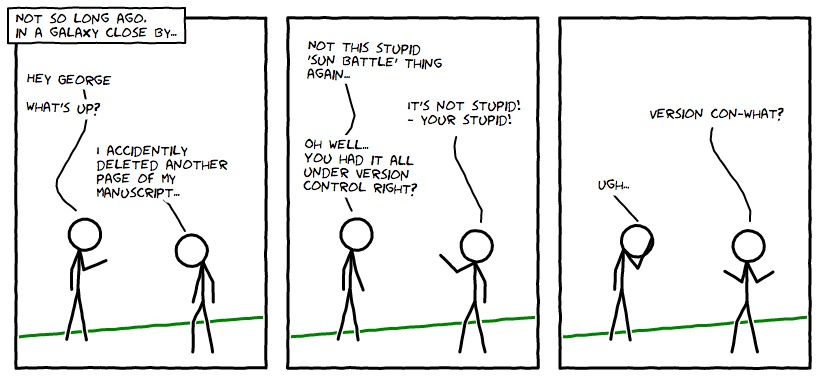
\includegraphics[width=1.0\linewidth]{figures/git-comics}
  \end{center}

\end{frame}

\begin{frame}
  \frametitle{What is Revision Control?}

  \begin{itemize}
    \item Management of changes to documents/code or any sorts of collections
      of information
    \item It is normally done by specialized software packages such as
      \texttt{git}
    \item There are two types:
      \begin{itemize}
        \item Centralized: Revision history is kept on a remote server
        \item Distributed: History is copied with the repository
      \end{itemize}
  \end{itemize}

  \begin{center}
    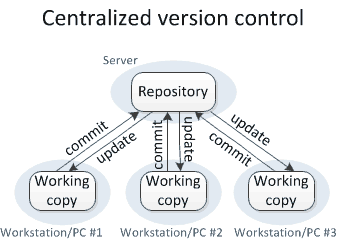
\includegraphics[width=0.45\linewidth]{figures/git-centralized}
    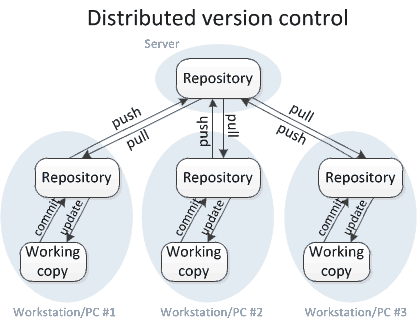
\includegraphics[width=0.45\linewidth]{figures/git-distributed}
  \end{center}

\end{frame}


\begin{frame}
  \frametitle{Why is it necessary?}

  Imagine a world w/o version control:

  \begin{itemize}
    \item You released version 1.0 of your software. It has a bug. Which other
      versions are affected?
    \item When was the last time I touched this file? Which changes did I do?
    \item You introduced a bug on the software: Where is that \textit{fracking}
      backup?
  \end{itemize}

  \begin{alertblock}{It is possible!}
    Actually, the Linux project stayed 11 years w/o version control!

    \vspace{1em}

    This was possible thanks to an ``extremely" organized procedure for
    diff/patching changes that gave birth to what is ``Git" today!
  \end{alertblock}

\end{frame}

\begin{frame}
  \frametitle{About Version Control}

  If you are a graphic or web designer and want to keep every version of an image or layout (which you would most certainly want to), a Version Control System (VCS) is a very wise thing to use. It allows you to:
  
  \begin{itemize}
   \item revert selected files back to a previous state, 
   \item revert the entire project back to a previous state, 
   \item compare changes over time, 
   \item see who last modified something that might be causing a problem, 
   \item who introduced an issue and when, and more. 
  \end{itemize}
\end{frame}

\subsection{Local vs Centralized vs Distributed VCS}

\begin{frame}
  \frametitle{Local Version Control Systems}
  One of the more popular VCS tools was a system called RCS, which is still distributed with many computers today. RCS works by keeping patch sets (that is, the differences between files) in a special format on disk; it can then re-create what any file looked like at any point in time by adding up all the patches.
  \vspace{1em}
  \begin{center}
    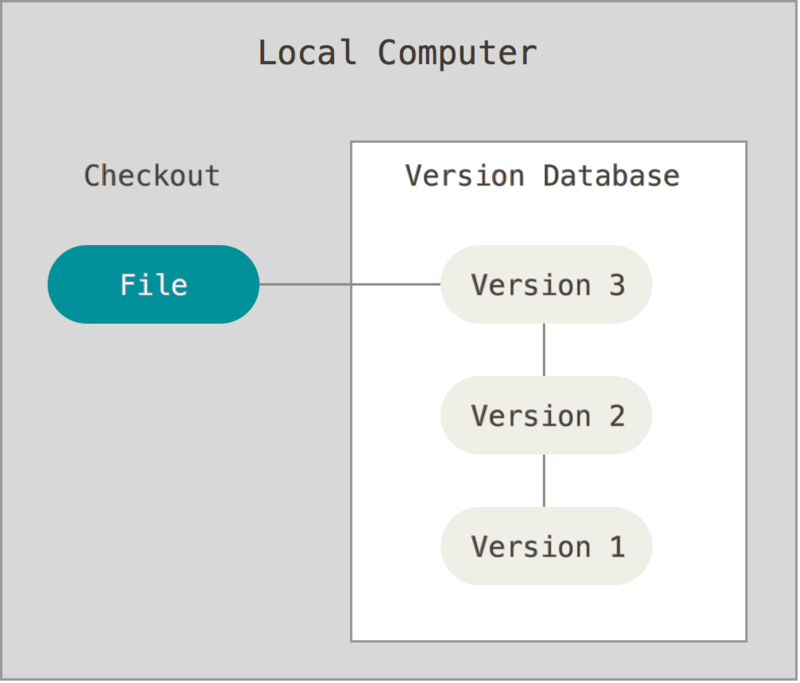
\includegraphics[width=0.5\linewidth]{figures/local}
  \end{center}
\end{frame}


\begin{frame}
  \frametitle{Centralized Version Control Systems (1)}
  The next major issue that people encounter is that they need to collaborate with developers on other systems. To deal with this problem, Centralized Version Control Systems (CVCSs) were developed. These systems (such as CVS, Subversion, and Perforce) have a single server that contains all the versioned files, and a number of clients that check out files from that central place. 
  \vspace{1em}
  \begin{center}
    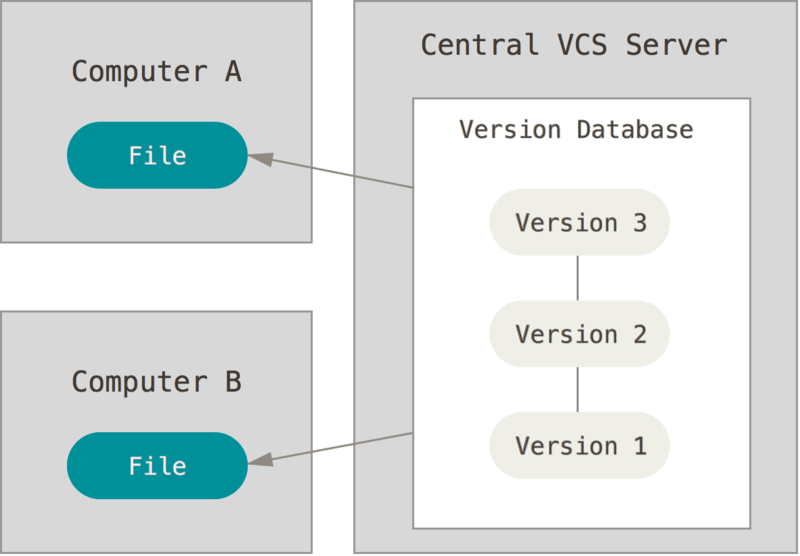
\includegraphics[width=0.5\linewidth]{figures/centralized}
  \end{center}
\end{frame}

\begin{frame}
  \frametitle{Centralized Version Control Systems (2)}
  This setup offers many advantages, especially over local VCSs.
  \begin{itemize}
   \item everyone knows to a certain degree what everyone else on the project is doing.
   \item Administrators have fine-grained control over who can do what, and it's far easier to administer a CVCS than it is to deal with local databases on every client. 
  \end{itemize}
  However, this setup also has some serious downsides:
  \begin{itemize}
   \item If that server goes down for an hour, then during that hour nobody can collaborate at all or save versioned changes to anything they're working on.
   \item If the hard disk the central database is on becomes corrupted, and proper backups haven't been kept, you lose absolutely everything-the entire history of the project.
  \end{itemize}
\end{frame}

\begin{frame}
  \frametitle{Distributed Version Control Systems}
  In a DVCS, such as Git, clients don’t just check out the latest snapshot of the files; rather, they fully mirror the repository, including its full history.
    \vspace{1em}
  \begin{center}
    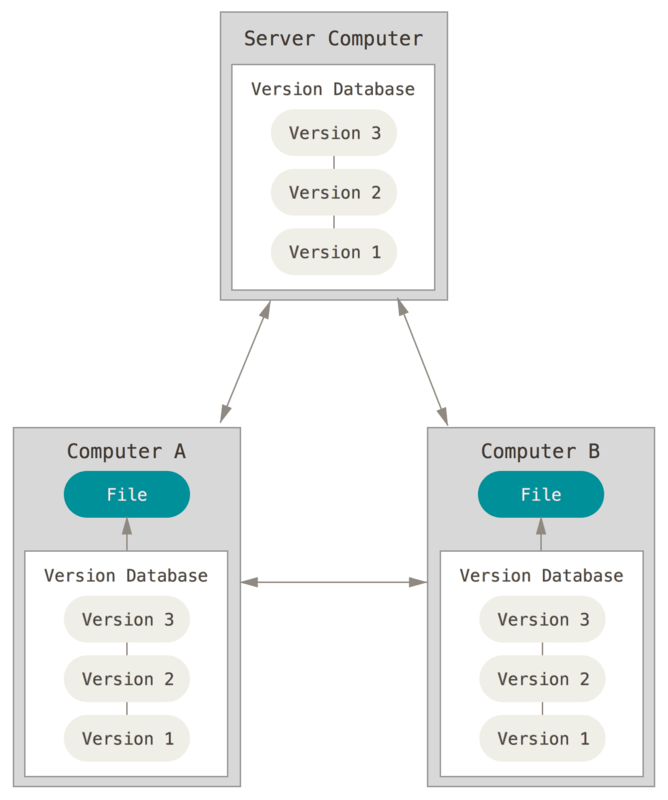
\includegraphics[width=0.5\linewidth]{figures/distributed}
  \end{center}
\end{frame}

\begin{frame}
  \frametitle{Distributed Version Control Systems}
   If any server dies, and these systems were collaborating via that server, any of the client repositories can be copied back up to the server to restore it. Every clone is really a full backup of all the data.
   Furthermore, many of these systems deal pretty well with having several remote repositories they can work with, so you can collaborate with different groups of people in different ways simultaneously within the same project. This allows you to set up several types of workflows that aren’t possible in centralized systems, such as hierarchical models.
\end{frame}

\subsection{Installing git}

\begin{frame}
\frametitle{Installing git}
The first step on the way to using Git is to install it! The directions found in the Git documentation below are pretty thorough and helpful, check them out for the best method of getting Git onto your platform of choice.

 \begin{itemize}
   \item \href{https://git-scm.com/downloads}{Git download page}
   \item \href{https://git-scm.com/book/en/v2/Getting-Started-Installing-Git}{Git installation instructions for each platform}
  \end{itemize}

\end{frame}

\subsection{Snapshots, Not Differences!}

\begin{frame}
  \frametitle{Snapshots, Not Differences}
  \begin{itemize}
   \item The major difference between Git and any other VCS (Subversion and friends included) is the way Git thinks about its data.
   \item most other systems store information as a list of file-based changes. 
  \end{itemize}
  
    \vspace{1em}
  \begin{center}
    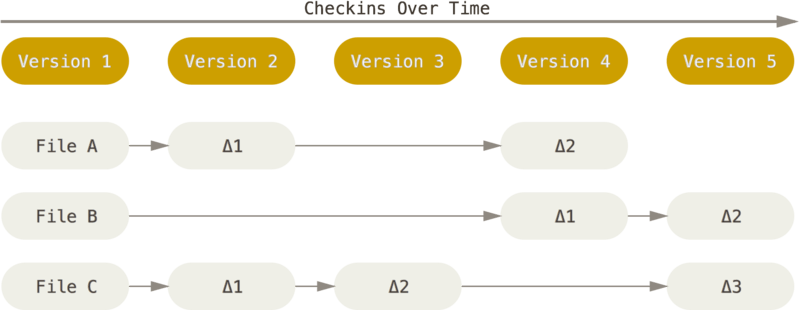
\includegraphics[width=0.8\linewidth]{figures/deltas}
  \end{center}
\end{frame}

\begin{frame}
  \frametitle{Snapshots, Not Differences}
  \begin{itemize}
   \item Git doesn’t think of or store its data this way. 
   \item Git thinks of its data more like a series of snapshots of a miniature filesystem. 
   \item Every time you commit, or save the state of your project, Git basically takes a picture of what all your files look like at that moment and stores a reference to that snapshot. 
   \item To be efficient, if files have not changed, Git doesn’t store the file again, just a link to the previous identical file it has already stored. 
   \item Git thinks about its data more like a \textbf{stream of snapshots}. 
  \end{itemize}
  
  \begin{center}
    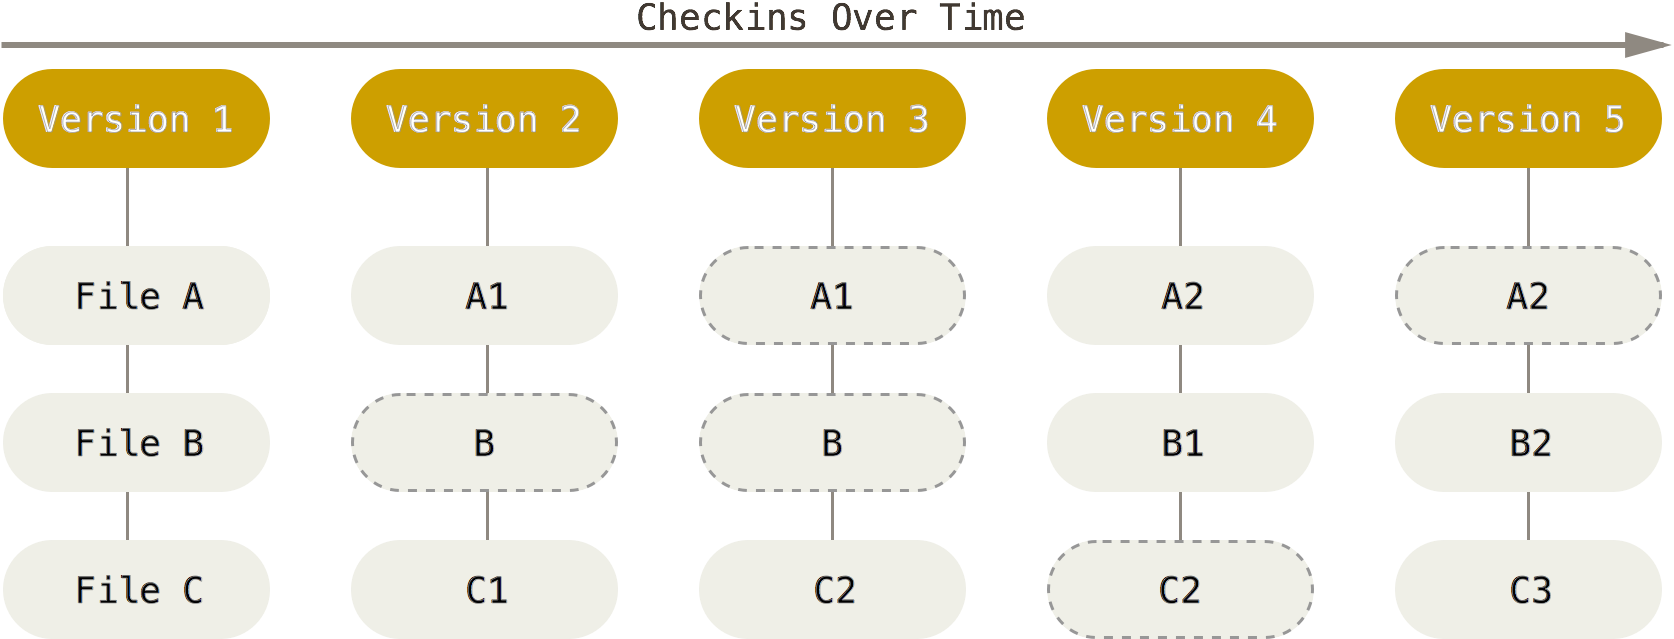
\includegraphics[width=0.8\linewidth]{figures/git-snapshots}
  \end{center}
\end{frame}



\begin{frame}
  \frametitle{Git}

  What is Git?

  \vspace{1em}

  Git is a distributed revision control system. It keeps \textbf{snapshots} of
  \textbf{the entirety} of your versioned directory through time using
  patches.

  \vspace{1em}

  \begin{center}
    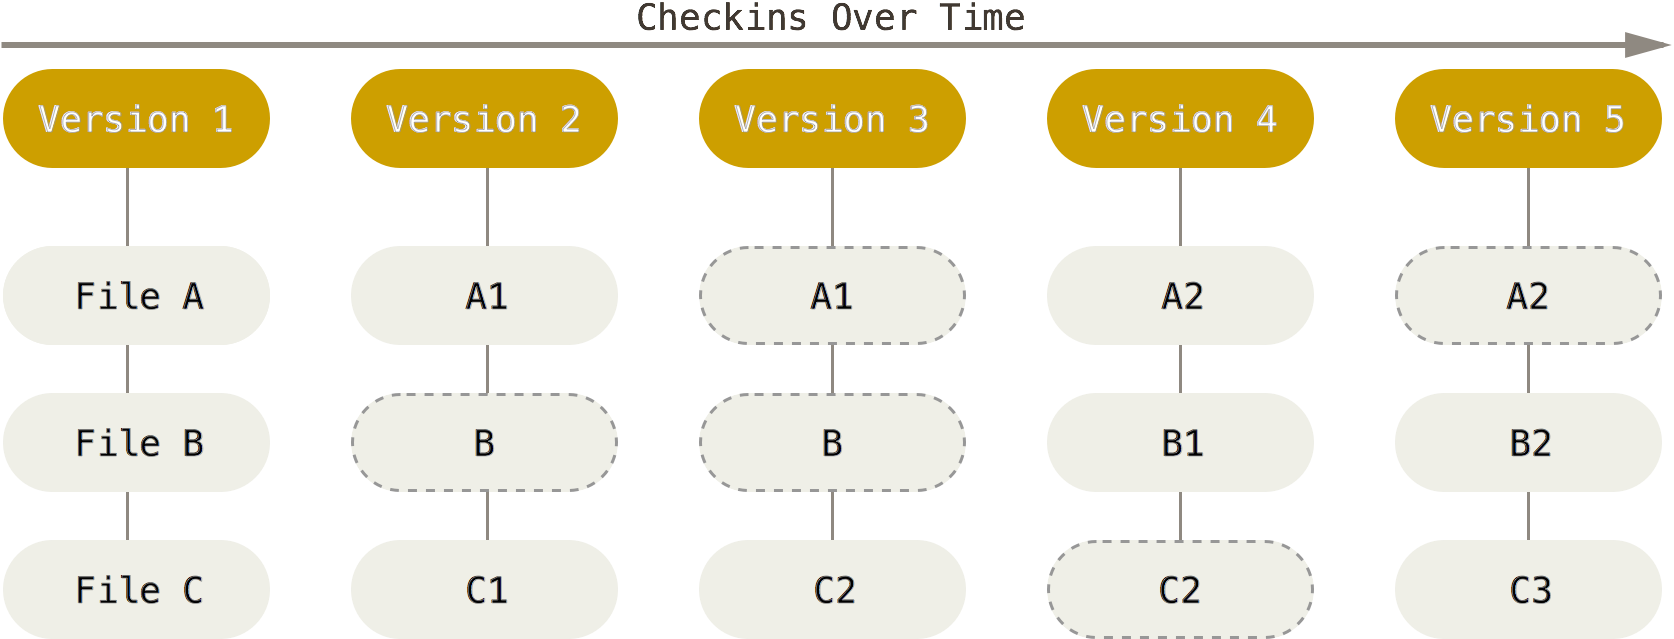
\includegraphics[width=0.8\linewidth]{figures/git-snapshots}
  \end{center}

  \only<2->{
    \begin{block}{Old tools, new usage}
      In order to create a snapshot, git uses \textit{diffs}, \textit{patches}
      and (SHA-1) \textit{hashes}
    \end{block}
  }

\end{frame}


\defverbatim[colored]\gitzeroone{
  \begin{textcode}
      file1.txt:                            file2.txt:

      I need to go to the store.            I need to go to the store.
      I need to buy some apples.            I need to buy some apples.
      When I get home, I'll wash the dog.   I also need to buy grated cheese.
                                            When I get home, I'll wash the dog.
  \end{textcode}
}

\defverbatim[colored]\gitzerotwo{
  \begin{shcode}
      $ diff file1.txt file2.txt > patch.txt
      $ cat patch.txt
      2a3
      > I also need to buy grated cheese.
  \end{shcode}
}

\begin{frame}
  \frametitle{\$h!tty situation!}

  \begin{center}
    
\includegraphics[width=0.6\linewidth]{figures/phdcomics}
  \end{center}

\end{frame}


\begin{frame}
  \frametitle{Diff/Patch}

  A \textit{diff} is a set of textual differences between files.

  \vspace{1em}

  \gitzeroone

  \vspace{1em}

  To create a \textit{patch}, use the \texttt{diff} command:

  \gitzerotwo

  \begin{exampleblock}{Translating}
    After line 2 in the first file, a line needs to be added: line 3 from the
    second file.
  \end{exampleblock}

\end{frame}


%*
\begin{frame}
  \frametitle{Applying patches (1)}

  Say you're receiving a \textit{diff} file, and you want to apply the changes. Do you know how to do it?
  \begin{itemize}
    \item You can do it manually (but what's the point?)
    \item You can use the command \textit{patch}
  \end{itemize}
  Let's say you wrote the following code:
  \includecode{codes_for_slides/cpu_usage.py}
  Then you noticed that there's something not correct so you asked a friend to help you!
\end{frame}

%*
\begin{frame}
  \frametitle{Applying patches (2)}

  Your friend sent you the following \textit{patch} file named \textit{cpu\_usage.diff}:
  \includecode{codes_for_slides/cpu_usage.diff}
  Do you notice what are the changes that your friend made? How to integrate them in your code?
\end{frame}

%*
\begin{frame}
  \frametitle{Applying patches (3)}

  To include the changes into your code \textit{cpu\_usage.py}, you can simply use the following command:
  \includebash{codes_for_slides/diff_cpu.sh}
  Then your code will be as follows:
  \includecode{codes_for_slides/cpu_usage1.py}
\end{frame}

\subsection{Hash}
\begin{frame}
  \frametitle{Hash}

  A (crypto) hash function is a function that can be used to map digital data
  of arbitrary size to a fixed length string, that is practically impossible to
  invert.

  \begin{center}
    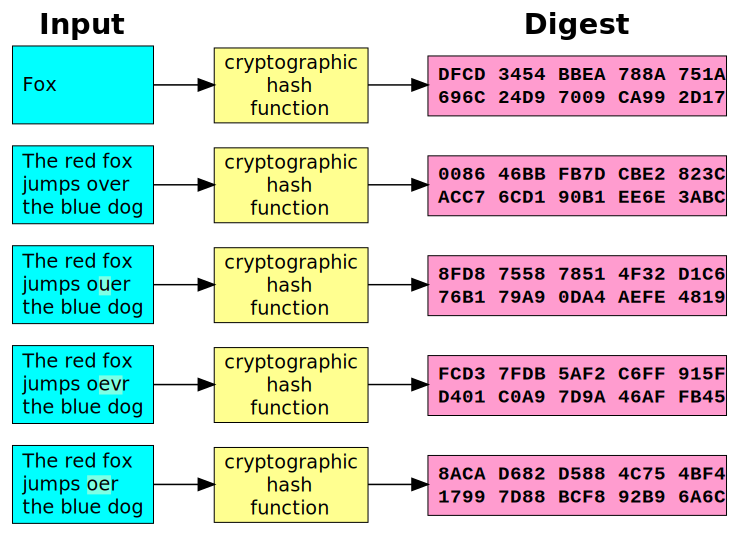
\includegraphics[width=0.6\linewidth]{figures/git-hash}
  \end{center}

  \vspace{1em}

  \textit{Notice that small changes on the input make the hash change a lot.}

\end{frame}


\begin{frame}
  \frametitle{Hash (collision)}

  \begin{block}{Nearly impossible to clash}
    It is nearly \textbf{impossible} that two natural sequences collide on the
    \textbf{same} repository.
  \end{block}

  \vspace{2em}

  If all world population would be developers and every one of them would
  commit to the \textbf{same} repository every second, the probability of 50\%
  collision would be reached in\footnote{http://diego.assencio.com/?index=eacd6eedf46c9dd596a5f12221ad15b8}:

  \[
    6.6 \times 10^6 \text{years}
  \]

\end{frame}

\subsection{Git states and workflow}

\begin{frame}
  \frametitle{Git states}

  Git contains 3 states for your project.

  \vspace{1em}

  \begin{center}
    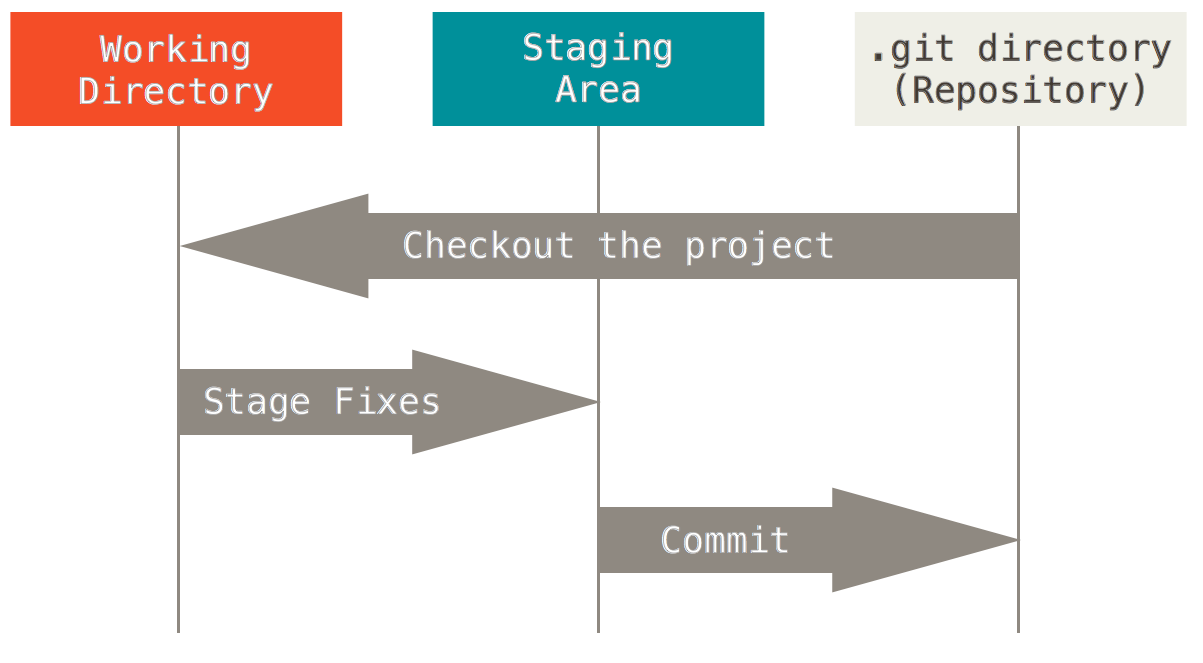
\includegraphics[width=0.9\linewidth]{figures/git-areas}
  \end{center}

\end{frame}


\begin{frame}

  \frametitle{Git workflow}

  Easy

  \vspace{2em}

  \begin{itemize}
    \item You modify files in your working directory.

    \item You stage the files, adding snapshots of them to your staging area.

    \item You do a commit, which takes the files as they are in the staging
      area and stores that snapshot permanently to your Git directory.
  \end{itemize}

\end{frame}


  \section{Git Basics}

% \defverbatim[colored]\gitone{
%   \begin{shcode}
%       $ cp -r ex4 myproj
%       $ cd myproj
%       $ git init
%       Initialized empty Git repository in ...
%   \end{shcode}
% }

\defverbatim[colored]\gitone{
  \begin{shcode}
      $ cd myproj
      $ git init
      Initialized empty Git repository in ...
  \end{shcode}
}


\defverbatim[colored]\gitonetwo{
  \begin{shcode}
      $ git config --global user.name "First Last"
      $ git config --global user.email first.last@example.com
      # to list all configuration set for you
      $ git config --list
    \end{shcode}
}

\subsection{Configuration and \texttt{init}}

\begin{frame}
  \frametitle{Configuring \texttt{git} (first time only)}

  To tell git it should log every commit using your name and e-mail, you need
  to configure it once:

  \vspace{2em}

  \gitonetwo

  \begin{exampleblock}{Tip}
    Tab-like auto-completion works out-of-the-box!
  \end{exampleblock}

\end{frame}


\begin{frame}
  \frametitle{Initializing a new repository}

  To initialize a repository just use \texttt{git init}. Let's try it!

  \vspace{2em}

  \gitone

\end{frame}


\defverbatim[colored]\gittwo{
  \begin{shcode}
      $ git status
      On branch master

      Initial commit

      Untracked files:
        (use "git add ...
  \end{shcode}
}

\begin{frame}
  \frametitle{What is staged?}

  The \texttt{status} command gives an overview of the staging area.

  \vspace{2em}

  \gittwo

\end{frame}


\defverbatim[colored]\gitthree{
  \begin{shcode}
      $ git add . #adds all files to staging area
      $ git commit -m "My first commit with git"
      $ git status
      On branch master
      nothing to commit, working directory clean
  \end{shcode}
}

\defverbatim[colored]\gitthreeone{
  \begin{shcode}
      $ git config --global core.editor /usr/bin/nano #default
      $ git config --global core.editor /usr/bin/gedit
      $ git config --global core.editor /usr/bin/vim
      $ git config --global core.editor /usr/bin/gvim
  \end{shcode}
}

\begin{frame}
  \frametitle{Let's do the first commit}

  The \texttt{commit} command instructs git to register the snapshot (patch) to
  its \texttt{.git} directory.

  \vspace{2em}

  \gitthree

  \begin{exampleblock}{Tip: Configuring the default editor}
      \gitthreeone
  \end{exampleblock}

\end{frame}


% \defverbatim[colored]\gitfour{
%   \begin{shcode}
%       $ gedit analysis.py #undo the change
%       # now we use git to problem for the modification
%       $ git diff
%       diff --git a/analysis.py b/analysis.py
%       index d4d5b3e..2697486 100644
%       --- a/analysis.py
%       +++ b/analysis.py
%       @@ -20,4 +20,4 @@ def CER(prediction, true_labels):
%          """

%          errors = (prediction != true_labels).sum()
%       -  return float(errors)/len(prediction)
%       +  return errors/len(prediction)
%   \end{shcode}
% }

\defverbatim[colored]\gitfour{
  \begin{shcode}
      $ #make some changes
      # now we use git to problem for the modification
      $ git diff
      diff --git a/analysis.py b/analysis.py
      index d4d5b3e..2697486 100644
      --- a/analysis.py
      +++ b/analysis.py
      @@ -20,4 +20,4 @@ def CER(prediction, true_labels):
         """

         errors = (prediction != true_labels).sum()
      -  return float(errors)/len(prediction)
      +  return errors/len(prediction)
  \end{shcode}
}

\subsection{Making changes and commits}

\begin{frame}
  \frametitle{Making changes}
  The power of version control can be shown when you make changes.
  % The power of version control can be shown when you make changes. Let's go
  % back to the file \texttt{analysis.py} and undo the fix you just did, so the
  % bug we corrected is re-introduced.

  \vspace{1em}

  \gitfour

  % \textcolor{red}{Note: The commit hashes my differ}

\end{frame}


\defverbatim[colored]\gitfive{
  \begin{shcode}
      $ git commit -m "Re-added nasty bug" -a
  \end{shcode}
}

\begin{frame}
  \frametitle{Committing changes (faster)}

  You can stage and commit changes with one command.

  \vspace{2em}

  \gitfive

\end{frame}


\defverbatim[colored]\gitsix{
  \begin{shcode}
      $ git log --oneline
      df7bc06 Re-added nasty bug
      ccb2d42 My first commit with git
      $ #figured out I re-added the bug, so will revert
      $ git revert df7bc06
      # edit the comment, and save (<ESC>:wq)
      $ git log --oneline
      a43f4c6 Revert "Re-added nasty bug"
      df7bc06 Re-added nasty bug
      ccb2d42 My first commit with git
      $ git diff df7bc06..a43f4c6
      # OK!
  \end{shcode}
}


\begin{frame}
  \frametitle{Recording Changes to the Repository}

  Each file in your working directory can be in one of two states: tracked or untracked.
  Tracked files are files that were in the last snapshot; they can be unmodified, modified, or staged.

  \vspace{1em}

  \begin{center}
    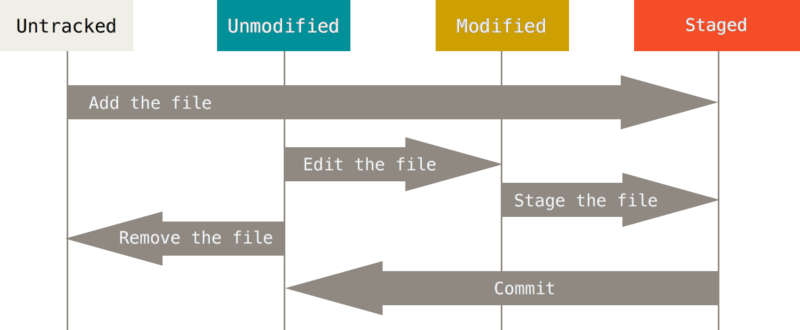
\includegraphics[width=0.9\linewidth]{figures/git-lifecycle}
  \end{center}

\end{frame}

\subsection{Logs, Diffs and Tags}

\begin{frame}
  \frametitle{Logs and Diffs}

  At all times, you have access to history and can revert back.

  \vspace{2em}

  \gitsix

\end{frame}


\defverbatim[colored]\gitseven{
  \begin{shcode}
      $ git tag final #makes final == a43f4c6..
      $ git tag buggy df7bc06 #makes buggy == df7bc06...
      $ git diff buggy..final
      ...
      $ git tag
      buggy
      final
  \end{shcode}
}


\begin{frame}
  \frametitle{Tags}

  Git allows you to set labels to refer to repository versions (instead of
  hash initials). You should use the \texttt{tag} command to do so.

  \vspace{2em}

  \gitseven

\end{frame}

\defverbatim[colored]\gitignore{
  \begin{shcode}
      $ cat .gitignore
      *.[oa]
      *~
  \end{shcode}
}

\subsection{Ignoring Files}
\begin{frame}
  \frametitle{Ignoring Files}

  Git allows you can create a file listing patterns that you want to ignore.
  \vspace{2em}

  \gitignore

  The first line tells Git to ignore any files ending in “.o” or “.a”
  The second line tells Git to ignore all files whose names end with a tilde ($\sim$).
\end{frame}


\begin{frame}
  \frametitle{Rules for \texttt{.gitignore}}

  The rules for the patterns you can put in the .gitignore file are as follows:
  \begin{itemize}
    \item Blank lines or lines starting with \# are ignored.
    \item Standard glob patterns work, and will be applied recursively throughout the entire working tree.
    \item You can start patterns with a forward slash (/) to avoid recursivity.
    \item You can end patterns with a forward slash (/) to specify a directory.
    \item You can negate a pattern by starting it with an exclamation point (!).
  \end{itemize}
\end{frame}

\defverbatim[colored]\gitignoreExample{
  \begin{shcode}
      # ignore all .a files
      *.a
      # but do track lib.a, even though you're ignoring .a files above
      !lib.a
      # only ignore the TODO file in the current directory,
      # not subdir/TODO
      /TODO
      # ignore all files in any directory named build
      build/
      # ignore doc/notes.txt, but not doc/server/arch.txt
      doc/*.txt
      # ignore all .pdf files in the doc/ directory and any of its 
      # subdirectories
      doc/**/*.pdf
  \end{shcode}
}

\begin{frame}
  \frametitle{Ignoring Files}

  Here is another example .gitignore file:

  \vspace{2em}

  \gitignoreExample

\end{frame}

\begin{frame}
  \frametitle{Viewing the Commit History}

  After you have created several commits, or if you have cloned a repository with an existing commit history, you’ll probably want to look back to see what has happened. The most basic and powerful tool to do this is the git log command.
  \vspace{2em}

\end{frame}


  \section{Branches}

\subsection{Branches in a Nutshell}

\begin{frame}
  \frametitle{Branches in a Nutshell (1)}
  \begin{itemize}
  \item When you make a commit, Git stores a commit object that contains a pointer to the snapshot of the content you staged.
  \item This object also contains the author’s name and email address, the message that you typed, and pointers to the commit or commits that directly came before this commit (its parent or parents)
  \end{itemize}
  \begin{center}
    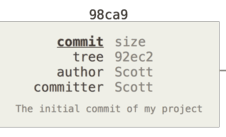
\includegraphics[width=0.7\linewidth]{figures/git-commit}
  \end{center}
commit-and-tree
\end{frame}

\defverbatim[colored]\gitcommit{
  \begin{shcode}
    $ git add README test.rb LICENSE
    $ git commit -m 'The initial commit of my project'
  \end{shcode}
}

\begin{frame}
  \frametitle{Branches in a Nutshell (2)}
  \begin{itemize}
  \item let’s assume that you have a directory containing three files, and you stage them all and commit.
  \item Staging the files computes a checksum for each one (the SHA-1 hash we mentioned before), stores that version of the file in the Git repository (Git refers to them as blobs), and adds that checksum to the staging area:
  \end{itemize}
\gitcommit
  \begin{itemize}
  \item When you create the commit by running git commit, Git checksums each subdirectory and stores those tree objects in the Git repository. 
  \item Git then creates a commit object that has the metadata and a pointer to the root project tree so it can re-create that snapshot when needed.
  \end{itemize}
\end{frame}

\begin{frame}
  \frametitle{Branches in a Nutshell (3)}
  Your Git repository now contains five objects:
  \begin{itemize}
  \item three blobs (representing the contents of one of the three files)
  \item one tree that lists the contents of the directory and specifies which file names are stored as which blobs
  \item one commit with the pointer to that root tree and all the commit metadata.
  \end{itemize}
  \vspace{-1em}
  \begin{center}
    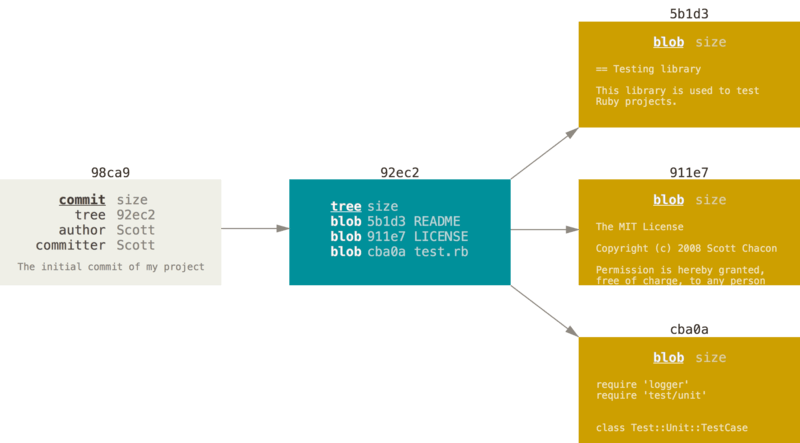
\includegraphics[width=0.9\linewidth]{figures/commit-and-tree}
  \end{center}
\end{frame}

\begin{frame}
  \frametitle{Branches in a Nutshell (4)}
If you make some changes and commit again, the next commit stores a pointer to the commit that came immediately before it.
  \vspace{1em}
  \begin{center}
    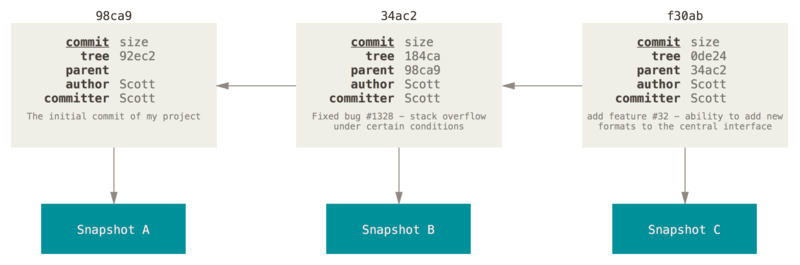
\includegraphics[width=\linewidth]{figures/commits-and-parents}
  \end{center}
\end{frame}

\subsection{Branches in action}

\begin{frame}
  \frametitle{Branches}

  A branch in Git is simply a lightweight movable pointer to one of these commits. By default, there is only one branch (called \texttt{master}) on a git repository.

  \begin{center}
    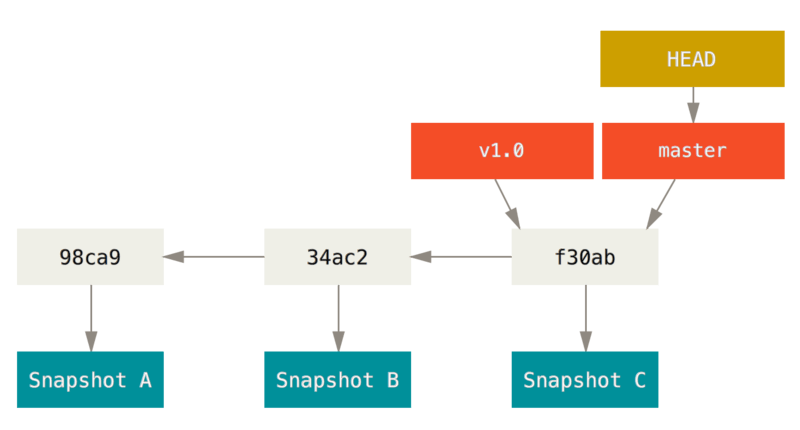
\includegraphics[width=\linewidth]{figures/branch-and-history}
  \end{center}

\end{frame}


\defverbatim[colored]\giteight{
  \begin{shcode}
      $ git branch testing
  \end{shcode}
}
\begin{frame}
  \frametitle{Branches (2)}

  You may create a new branch, to develop something new while keeping the
  master stable.

  \vspace{1em}

  \giteight

  \begin{center}
    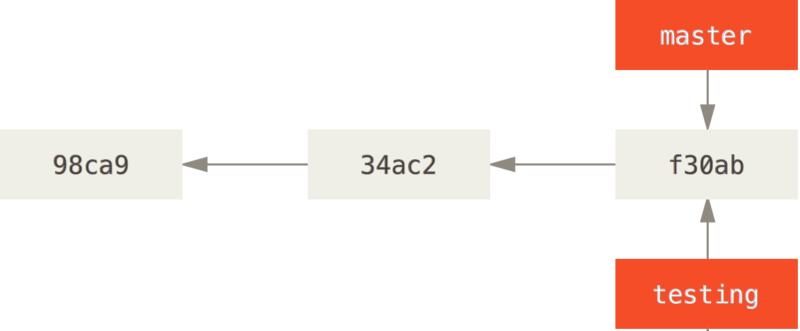
\includegraphics[width=0.9\linewidth]{figures/git-two-branches}
  \end{center}

\end{frame}

\begin{frame}
  \frametitle{Branches (3)}

  How does Git know what branch you’re currently on?\\
  It keeps a special pointer called \texttt{HEAD}

  \begin{center}
    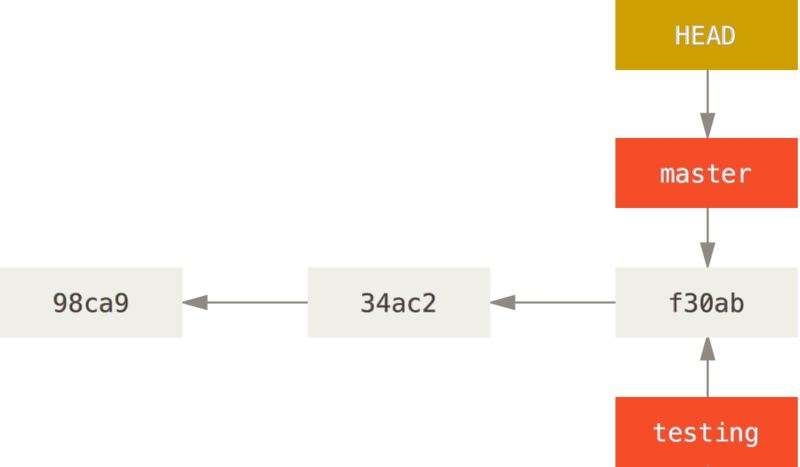
\includegraphics[width=0.7\linewidth]{figures/head-to-master}
  \end{center}
  
  \begin{alertblock}{Pay attention!}
    The git branch command only created a new branch - it didn't switch to that branch.
  \end{alertblock}
\end{frame}


\defverbatim[colored]\gitdecorate{
  \begin{shcode}
      $ git log --oneline --decorate
      f30ab (HEAD -> master, testing) add feature #32 - ability to add
      # new formats to the central interface
34ac2 Fixed bug #1328 - stack overflow under certain conditions
98ca9 The initial commit of my project
  \end{shcode}
}
\begin{frame}
  \frametitle{Branches (4)}

   You can easily see on which branch the \texttt{HEAD} is pointing by running a simple \texttt{git log} command that shows you where the branch pointers are pointing. This option is called \texttt{--decorate}.

  \gitdecorate
\end{frame}



\defverbatim[colored]\gitnine{
  \begin{shcode}
      $ git checkout testing
      Switched to a branch "testing"
  \end{shcode}
}

\subsection{Switching Branches}
\begin{frame}
  \frametitle{Switching Branches}

  To tell Git to consider a new branch as the default for commiting, use the
  \texttt{checkout} command:

  \gitnine

This moves \texttt{HEAD} to point to the \texttt{testing} branch.

\begin{center}
    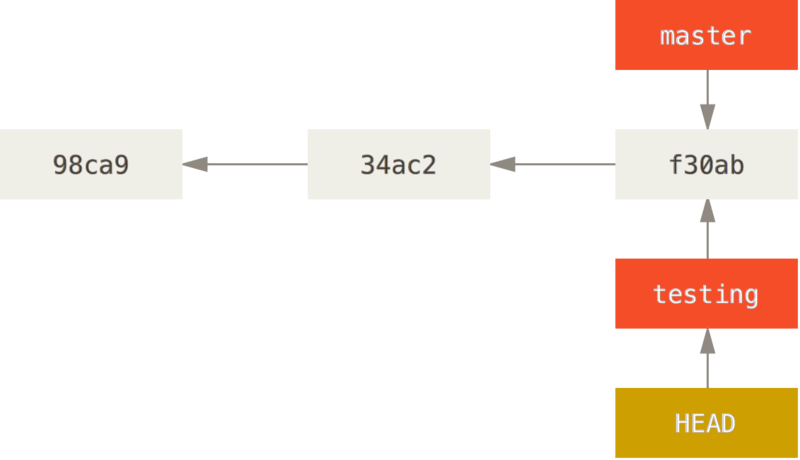
\includegraphics[width=0.7\linewidth]{figures/head-to-testing}
  \end{center}

\end{frame}


\defverbatim[colored]\gitcommitbranch{
  \begin{shcode}
      $ vim test.rb
      $ git commit -a -m 'made a change'
  \end{shcode}
}

\begin{frame}

  \frametitle{Switching Branches (2)}

  If you commit a change, only the marker \texttt{testing} will be modified:

  \gitcommitbranch

  \begin{center}
    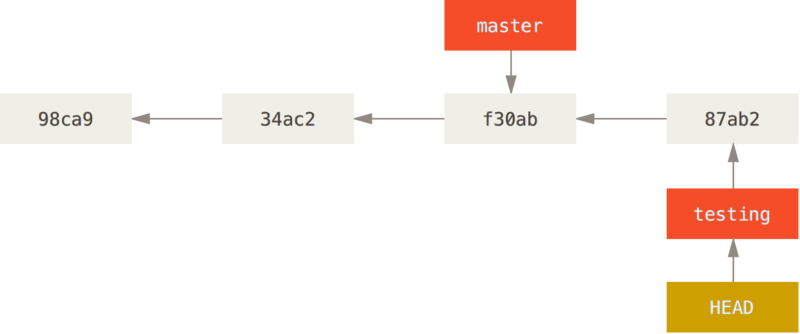
\includegraphics[width=0.8\linewidth]{figures/advance-testing}
  \end{center}

\end{frame}

\defverbatim[colored]\gitcheckoutmaster{
  \begin{shcode}
      $ git checkout master
  \end{shcode}
}
\begin{frame}
  \frametitle{Switching Branches (3)}

  If you commit a change, only the marker \texttt{testing} will be modified:

  \gitcheckoutmaster
  \vspace{-1em}
  \begin{center}
    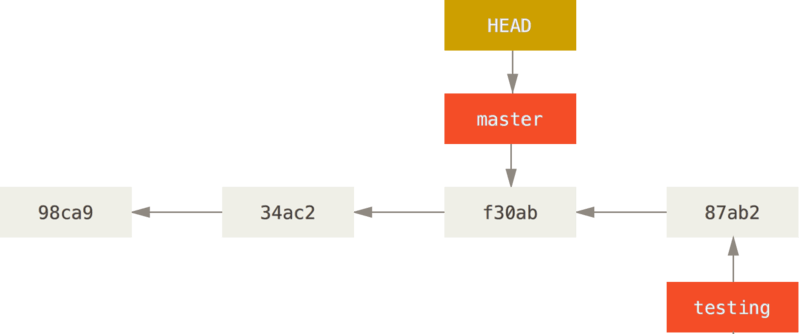
\includegraphics[width=0.7\linewidth]{figures/checkout-master}
  \end{center}
  \begin{alertblock}{Pay attention!}
  That command did two things. It moved the \texttt{HEAD} pointer back to point to the \texttt{master} branch, and it reverted the files in your working directory back to the snapshot that master points to. 
  \end{alertblock}
\end{frame}

\defverbatim[colored]\gitmorechanges{
  \begin{shcode}
      $ vim test.rb
      $ git commit -a -m 'made other changes'
  \end{shcode}
}
\begin{frame}
  \frametitle{Switching Branches (4)}
  Let’s make a few changes and commit again:
  \gitmorechanges
  \vspace{-1em}
  \begin{center}
    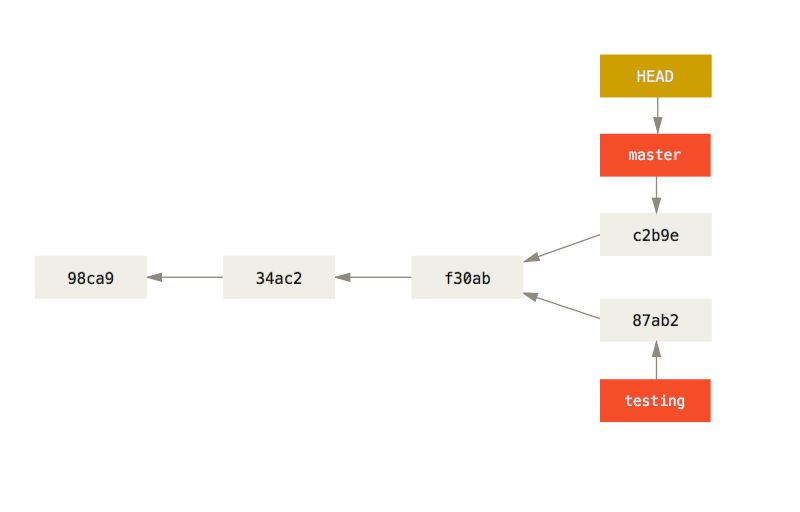
\includegraphics[width=\linewidth]{figures/advance-master}
  \end{center}
\end{frame}


\defverbatim[colored]\gitten{
  \begin{shcode}
      $ gedit ...
      $ git commit -m "My change to the special branch" -a
      $ git log --oneline #has the new commit
      ...
      $ git log --oneline master #as before
      ...
      $ git checkout master #To go back to the master
      $ git merge testing #To merge all changes back
      $ git branch -d testing #To remove the branch
  \end{shcode}
}
\begin{frame}
  \frametitle{Switching Branches: some commands}
  \vspace{2em}
  \gitten
\end{frame}

\defverbatim[colored]\giteleven{
  \begin{shcode}
      $ git branch old-release tag-1.2.4
      $ git checkout old-release #state of version 1.2.4
      # edit the changes
      $ git commit -m "..."
      # release version 1.2.5 from that point
  \end{shcode}
}

\begin{frame}
  \frametitle{How to Properly Use Tag/Branches}

  As rule of thumb:

  \vspace{1em}

  \begin{itemize}
    \item Everytime you make a \textbf{new release}, you \textbf{tag} your
      repository so you know what was distributed
    \item You use branches to:
      \begin{itemize}
        \item Test new features w/o disturbing the stability of \texttt{master}
        \item Fix problems with old versions of the software:

          \vspace{1em}
          \giteleven
      \end{itemize}
  \end{itemize}
\end{frame}

  
\section{More about Git}

\begin{frame}
  \frametitle{More Git}

  Here is a list of resources if you're interested to know more about this
  powerful tool:

  \vspace{2em}

  \begin{itemize}
    \item Reference website: \url{https://git-scm.com/documentation}
      \begin{itemize}
        \item Detailed tutorials
        \item Videos
        \item Reference documentation
      \end{itemize}
      videos)
    \item ProGit Book (2nd Edition): \url{http://git-scm.com/book/en/v2}
    \item MOOC: \url{https://www.codeschool.com/courses/try-git}
    \item YouTube clips from GitLab: \url{https://www.youtube.com/channel/UCnMGQ8QHMAnVIsI3xJrihhg}
  \end{itemize}
\end{frame}

\begin{frame}
  \frametitle{GitLab: Push the code}

  You can now push your local code to the remote repository.

\end{frame}



\begin{frame}
  \frametitle{What to do?}

  Here is a list of tips:

  \vspace{2em}

  \begin{itemize}
    \item \textbf{Always} keep your source code under revision control
    \item \textbf{Commit} often
    \item \textbf{Tag} to keep track of important moments (paper status for example)
    \item Use \textbf{Branches} to apply fixes to distributed software
    \item Use GitLab as much as you can to host your code. It is free, robust and requires no maintenance efforts from you!
  \end{itemize}

\end{frame}

\end{document}
